% Name: Activity diagram
% Description: Handling an order as a UML activity diagram: actions, a decision with its guards, a fork and a join for work done in parallel, and the final node.
% Tags: activity diagram, UML, workflow, fork and join

\usetikzlibrary{arrows.meta, positioning, shapes.geometric}

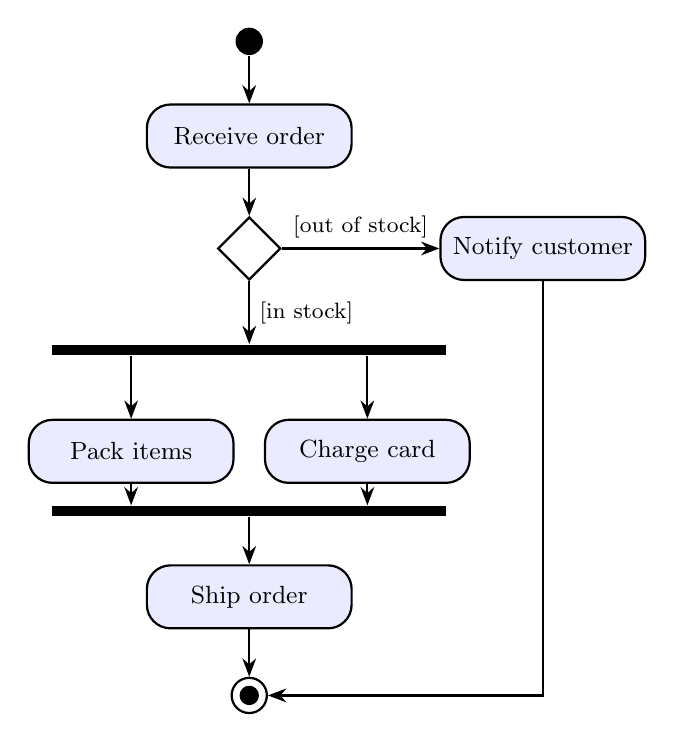
\begin{tikzpicture}[>={Stealth}, thick, node distance=6mm, every node/.style={font=\small},
    action/.style={draw, rounded corners=3mm, fill=blue!8, minimum width=26mm, minimum height=8mm},
    decision/.style={diamond, draw, fill=white, inner sep=0pt, minimum size=8mm},
    bar/.style={fill, minimum width=50mm, minimum height=1.2mm, inner sep=0pt}, guard/.style={font=\footnotesize}]
  \node[circle, fill, inner sep=3.5pt] (start) {};
  \node[action, below=of start] (receive) {Receive order};
  \node[decision, below=of receive] (stock) {};
  \node[action, right=20mm of stock] (notify) {Notify customer};
  \node[bar, below=8mm of stock] (fork) {};
  \node[action, below=8mm of fork, xshift=-15mm] (pack) {Pack items};
  \node[action, below=8mm of fork, xshift=15mm] (charge) {Charge card};
  \node[bar, below=19mm of fork] (join) {};
  \node[action, below=of join] (ship) {Ship order};
  \node[circle, draw, inner sep=4.5pt, below=of ship] (end) {};
  \fill (end) circle (3.5pt);
  \draw[->] (start) -- (receive);
  \draw[->] (receive) -- (stock);
  \draw[->] (stock) -- node[guard, above] {[out of stock]} (notify);
  \draw[->] (stock) -- node[guard, right] {[in stock]} (fork);
  \draw[->] (fork.south -| pack) -- (pack);
  \draw[->] (fork.south -| charge) -- (charge);
  \draw[->] (pack) -- (join.north -| pack);
  \draw[->] (charge) -- (join.north -| charge);
  \draw[->] (join) -- (ship);
  \draw[->] (ship) -- (end);
  \draw[->] (notify) |- (end);
\end{tikzpicture}
